\chapter{DevOps\label{devops}}

DevOpsilla tarkoitetaan ohjelmistokehityksen ja IT-toimintojen yhdistämistä.
DevOpsiin liitetään usein jatkuva integraatio ja toimitus sekä automaatio ja laadunvalvonta \cite{Jabbari16, Leite19}.
DevOpsia käsitteenä voidaan tarkastella ajattelutapana tai käytännön ohjelmistotuotannon toimintamallina.

DevOps ajattelutapana pyrkii ohjelmistokehityksen ja IT-toimintojen jaon välttämiseen ja yhteistoiminnan mahdollistavan kulttuurin rakentamiseen \cite{Klein21}.
DevOps toimintamallina taas keskittyy käytännön toimiin ja teknologioihin, jotka mahdollistavat DevOps-ajattelutavan mukaisen ohjelmistotuotannon.
Tässä tutkielmassa keskitytään aiheen käsittelyyn käytännön toimintamallin kautta.

\section{DevOps-toimintamalli}

DevOps-toimintamalli painottaa jatkuvaa integraatiota ja toimitusta sekä laadunvalvontaa käyttäen standardisoituja automaattisia menetelmiä \cite{Leite19}.
Kuva~\ref{fig:devops} visualisoi DevOps-toimintamallin eri vaiheita.
Kehitys- ja operaatiovaiheet tapahtuvat limittäin ja koko prosessi voidaan suorittaa useita kertoja päivässä automatisoidun julkaisuputken avulla.

\begin{figure}[ht]
\begin{center}
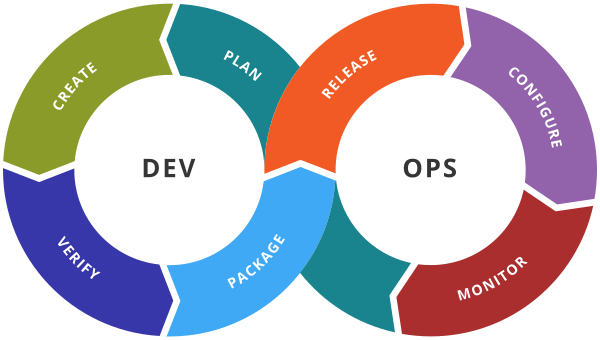
\includegraphics[width=0.6\textwidth]{figures/devops_toolchain.png}
\caption{DevOps-toimintamallin vaiheet \cite{Wikimedia23}\label{fig:devops}.}
\end{center}
\end{figure}

DevOps-toimintamallin vaiheet ja niistä käytetyt termit vaihtelevat lähteestä riippuen, mutta tämän tutkielman osalta käytetään seuraavia vaiheita \cite{Alnafessah21}:

\begin{itemize}
\item Määrittely (\textit{plan}): Ohjelmistotuotannon tavoitteiden määrittely sekä päivitysten ja julkaisuiden alustava suunnittelu.
\item Kehitys (\textit{create, develop}): Määrittelyn mukainen ohjelmisto- ja infrastruktuurikoodin kehitys nopealla versiohallintaan viennillä.
\item Varmennus (\textit{verify, test}): Jatkuva koodin automaattinen testaus ja koodin manuaalinen arviointi tarvittaessa.
\item Julkaisu (\textit{release, deploy}): Uuden ohjelmakoodin julkaisu tuotantoympäristöön ja tuotantoalustan konfiguraatio.
\item Operointi (\textit{operate, configure}): Julkaisun jälkeinen palvelun hallinnointi, resurssien hallinta ja palvelun skaalautuminen.
\item Monitorointi (\textit{monitor}): Palvelun suorituskyvyn ja lokien seuranta, ongelmatilanteisiin reagointi.
\end{itemize}

\section{Jatkuva integraatio ja toimitus}

Jatkuva integraatio ja toimitus (\textit{continuous integration and continuous delivery}) on keskeinen osa DevOps-toimintamallia \cite{Jabbari16, Leite19}.
Jatkuvan integraation ja toimituksen avulla voidaan automatisoida DevOps-toimintamallin varmennus- ja julkaisuvaiheet.

Jatkuva integraatio tarkoittaa koodimuutosten vientiä versionhallintaan nopealla tahdilla ja automaattista testausta koodimuutosten jälkeen.
Jatkuva toimitus taas tarkoittaa jatkuvan integraation jälkeen tapahtuvaa koodin automaattista julkaisua tuotantoympäristöön tai sitä muistuttavaan testiympäristöön \cite{Shahin17}.
Jatkuva integraatio ja toimitus mahdollistaa näin tehokkaan laadunvalvonnan ja ohjelmiston nopean julkaisusyklin.

\begin{figure}[ht]
\begin{center}
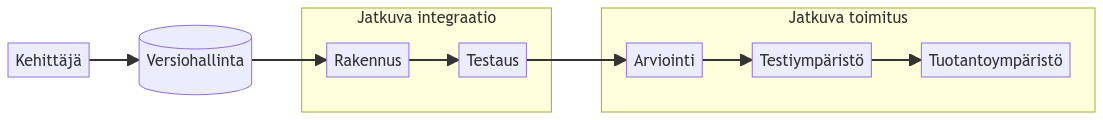
\includegraphics[width=1\textwidth]{figures/cicd-pipeline.png}
\caption{Jatkuvan integraation ja toimituksen vaiheet.\label{fig:cicd}}
\end{center}
\end{figure}

Kuva \ref{fig:cicd} esittää esimerkin jatkuvan integraation ja toimituksen vaiheista.
Jatkuva integraatio ja toimitus käynnistyy kehittäjän viedessä uuden koodimuutoksen versiohallintaan.
Jatkuvan integraation aikana uusi version sovelluksesta rakennetaan päivitetystä koodista ja uudelle versiolle suoritetaan automaattiset testit.
Automaattiset testit läpäissyt koodi voidaan tarvittaessa katselmoida ja sovelluksen uusi versio julkaistaan vaiheittain testi- ja tuotantoympäristöihin osana jatkuvaa toimitusta.

\section{Haasteet}

DevOps-toimintamalliin perustuva ohjelmistotuotanto luo uusia haasteita.
Haasteissa painottuvat erityisesti inhimilliset tekijät kuten kommunikaatiohaasteet ja muutosvastarinta \cite{Kalliosaari16}.
DevOps-toimintamallin käyttöönotto ja ohjelmistokehittäjien perehdyttäminen sen mukaisiin toimintatapoihin ja teknologioihin on haastavaa \cite{Leite19}.
Tässä tutkielmassa keskitytään kuitenkin DevOps-toimintamalliin liittyviin teknisiin haasteisiin.

Jatkuva integraatio ja toimitus sekä toimintamallin vaiheiden seuraaminen nopealla syklillä vaatii automaatiota ja vaiheiden helppoa toistettavuutta \cite{Jabbari16, Leite19}.
Teknisenä haasteena on myös ohjelmistoinfrastruktuurin kehittäminen ja hallinnointi, kuten monimutkaiset kehitys- ja tuotantoympäristöt \cite{Khan22, Kalliosaari16}.
Järkevien teknologiaratkaisujen valinta on toimintamallin onnistuneen käyttöönoton ja seurannan kannalta tärkeää.

DevOps-toimintamallin käyttöönoton yhteydessä on arvioitava erilaisten teknologioiden soveltuvuutta osaksi mallin mukaista ohjelmistotuotantoa.
Sopivilla teknologiavalinnoilla voidaan vähentää ohjelmistoinfrastruktuurin monimutkaisuutta.
Yksi näistä teknologiavalinnoista on julkaisutavan valinta.
Automaation ja toistettavuuden kannalta ratkaisuksi sopisi esimerkiksi virtuaalikoneet tai konttiteknologia \cite{Dua14}.
Konttiteknologiaa ja konttien orkestrointia voidaan käyttää onnistuneesti osana DevOps-toimintamallia \mbox{\cite{Kang16, Narasimhulu23}}.
Seuraavaksi käsitellään näitä aiheita ja arvioidaan niiden yhteensopivuutta DevOps-toimintamallin kanssa.

